\documentclass[UTF8]{ctexbeamer}
\usetheme{Madrid}
%\usecolortheme{beaver}
\usepackage{graphicx}
\DeclareGraphicsExtensions{.eps,.ps,.jpg,.bmp,.png}
%%Information to be included in the title page:
%\title{X}
%\author{Deli}
%%\institute{Deli institute}
%\date{\today}
\title[一维非线性方程的求根] %optional
{一维非线性方程的求根探讨}
% [] {} 两个还是有区别的,具体的差异尝试编译一下就了解了。

\usepackage{graphicx}
\usepackage{float}
\usepackage{subfigure}
\usepackage{amsmath}
\usepackage{amsfonts}
\usepackage{amsthm}
\usepackage{xcolor}
\usepackage[backref]{hyperref}
\usepackage{tikz}
\usepackage{ctex}
\usepackage{amssymb}
\usepackage{wasysym}
\usetikzlibrary{shapes,positioning}
\usepackage{listings}
\tikzstyle{inout}=  [draw,
trapezium,
trapezium left angle = 65,
trapezium right angle = 115,
trapezium stretches,
] %%输入输出框
\tikzstyle{endn}=   [draw,
rounded rectangle,
]   %%起止框
\tikzstyle{exec}=   [draw,
rectangle,]    %%执行框 execute
\tikzstyle{judge}= [draw,
diamond,
inner sep=0,]   %%判断框
\lstset{
    basicstyle          =   \sffamily,          % 基本代码风格
    keywordstyle        =   \bfseries,          % 关键字风格
    commentstyle        =   \rmfamily\itshape,  % 注释的风格,斜体
    stringstyle         =   \ttfamily,  % 字符串风格
    flexiblecolumns,
    breaklines          =   true, %对过长的代码自动换行
    numbers             =   left,   % 行号的位置在左边
    showspaces          =   false,  % 是否显示空格,显示了有点乱,所以不现实了
    numberstyle         =   \zihao{-5}\ttfamily,    % 行号的样式,小五号,tt等宽字体
    showstringspaces    =   false,
    captionpos          =   t,      % 这段代码的名字所呈现的位置,t指的是top上面
    frame               =   lrtb,   % 显示边框
}



\author{杨泽加 \\ 统计学 3190104662}

\institute[ZJU] % (optional)
{
    ZJU\\
    Statistics class 1901
}


%在每个section 前边单独插入当前章节高亮的目录页(当然最原始的目录页你还是需要手动录入的,不要想偷懒)
\AtBeginSection[]
{
    \begin{frame}
        \frametitle{Table of Contents}
        \tableofcontents[currentsection]
    \end{frame}
}

\begin{document}
    \maketitle
    \begin{frame}
        \frametitle{目录}
        目录:
        \begin{itemize}
            \item 导言
            \item 数学理论
            \item 算法介绍
            \item 两种算法收敛性的比较
            \item 结果分析
        \end{itemize}
    \end{frame}
    \begin{frame}
        \frametitle{导言}
        对一维非线性方程的求根,算法库 gsl 为我们提供了二分法、牛顿法及 Steffenson
        加速收敛法等不同方法。
        接下来我们将结合二分法和牛顿法展开讨论。
        由于所有一维非线性方程    \\
        \begin{equation}
            \label{E1}
            f(x) = b, b \in \mathbb{C} \Rightarrow g(x) = f(x) - b = 0
        \end{equation}
        也是一个一维非线性方程,所以一维非线性方程的解总是可以转化为一维线性方程的求根问题。
    \end{frame}
    \begin{frame}
        \frametitle{数学理论}
        \framesubtitle{二分法}
        对一个区间内单调的函数,若函数有实根,则函数曲线应当在根$x*$这一点上与
        x轴有一个交点,并且由于函数是单调的,在根附近的左右区间内,函数值的符号应当相反。
        利用这一特点,可以通过不断将求根区间二分的方法,每次将求根区间缩小为原来的一半,
        在新的折半后的区间内继续搜索方程的根,对根所在区间继续二分,直到求出方程的根为止。 \\
        这个算法的合理性由中值定理保证:\\
        \begin{theorem}[中值定理]
            \label{T1}
            设函数 $f$ 在闭区间 $[a,b]$ 内连续且在开区间 $(a,b)$ 可微,则存在一点
            $c, a < c < b$,使得
            \begin{equation}
                \label{E2}
                f'(c) = \frac{f(b) - f(a)}{b - a}.
            \end{equation}
        \end{theorem}
    \end{frame}
    \begin{frame}
        \frametitle{数学理论}
        \framesubtitle{牛顿法}
        牛顿法的基本思想是利用迭代点$x_k$处的一阶导数(梯度)和二阶导数(Hessen矩阵)
        对目标函数进行二次函数近似,然后把二次模型的极小点作为新的迭代点,并不断重复这一过程,
        直至求得满足精度的近似极小值。牛顿法的速度相当快,而且能高度逼近最优值。\\
        将 $f(x)$ 在 $x_0$ 点附近展开成 Taylor 级数\\
        \begin{equation}
            \label{E3}
            f(x) = f(x_0) + (x-x_0)f'(x_0) + (x-x_0)^2\frac{f''(x_0)}{2!} + \cdots
        \end{equation}
        取其线性部分作为非线性方程 $f(x) = 0$ 的近似方程,则有\\
        \begin{equation}
            \label{E4}
            f(x_0) + f'(x_0)(x-x_0) = 0
        \end{equation}
        设 $f'(x_0)\neq 0$,则其解为\\
        \begin{equation}
            \label{E5}
            x_1 = x_0 - \frac{f(x_0)}{f'(x_0)}
        \end{equation}
    \end{frame}
    \begin{frame}
        \frametitle{算法介绍}
        \begin{figure}[H]
            \centering
            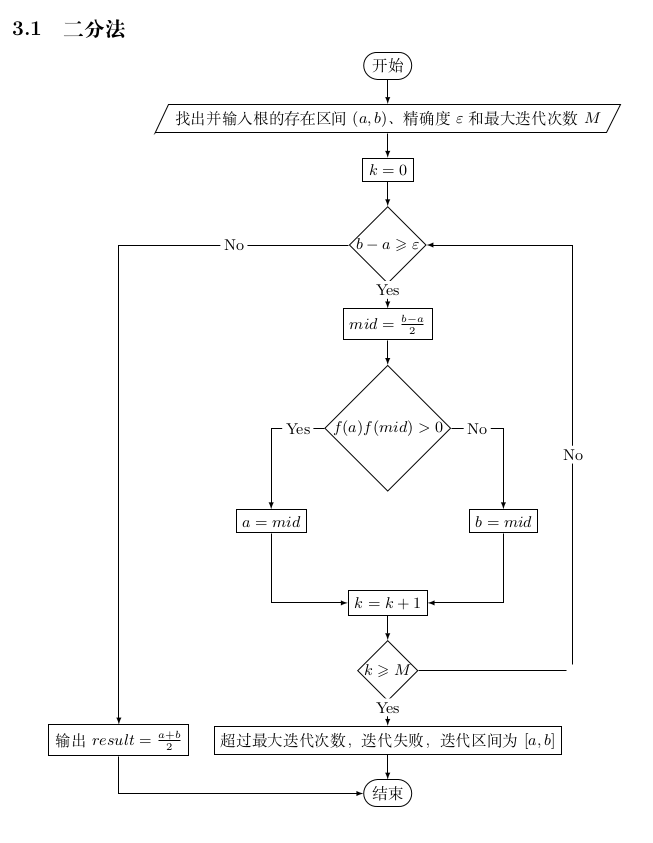
\includegraphics[scale=0.22]{dichotony}
            \caption{二分法的算法流程图}
        \end{figure}
    \end{frame}
    \begin{frame}
        \frametitle{算法介绍}
        \begin{figure}[H]
            \centering
            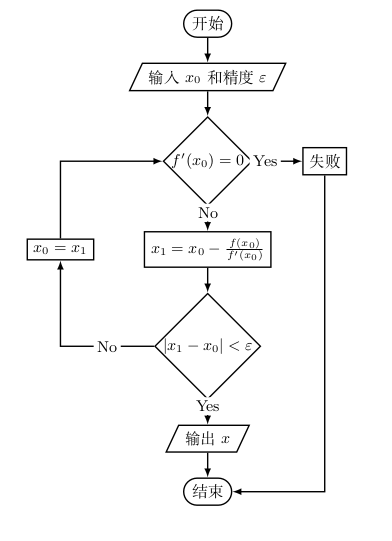
\includegraphics[scale=0.32]{Newton}
            \caption{牛顿的算法流程图}
        \end{figure}
    \end{frame}
    \begin{frame}[fragile]
        \frametitle{两种算法收敛性的比较}
        比较两种方法对1——10000的数字的求平方根结果如下:
        \begin{lstlisting}
10000次二分法迭代用时为850毫秒
10000次牛顿法迭代用时为1662毫秒
        \end{lstlisting}
        迭代次数的差异如下:
        \begin{figure}[H]
            \centering
            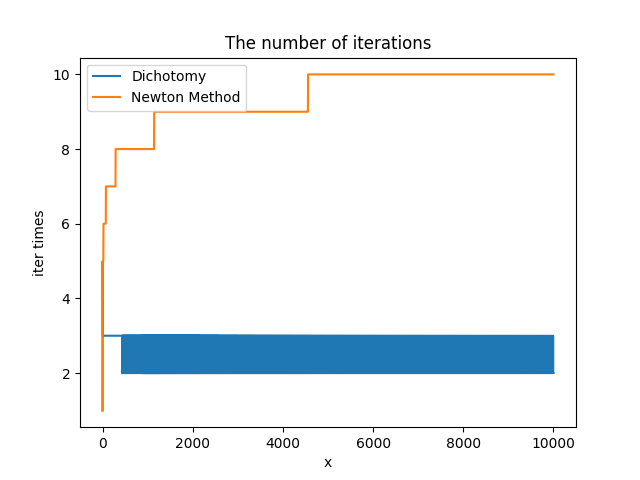
\includegraphics[scale=0.3]{./src/item}
        \end{figure}
    \end{frame}
    \begin{frame}
        \frametitle{结果分析}
        由于迭代的起始区间均为迭代区域的最大值 $\max(a,b)$。牛顿法对初值较为敏感,故迭代次数较多。
        而在起初区间较小时,牛顿法的效果则好于二分法。\\
        因此我们在根的估计区间较小时使用牛顿法,否则建议使用二分法。
    \end{frame}
\end{document}